\documentclass[12pt, a4paper]{report}

\usepackage{elegant-cours}

\begin{document}

\MaPageDeGarde{
    Chapitre III : Nombres Réels
}{
    Rédigé par Samy Youssoufine
}{
    ./assets/logo.png
}{}


\tableofcontents
\clearpage

\chapter{Borne supérieure et inférieure}
\begin{definition}
    Soit \(A\) une partie non vide de \(\mathbb{R}\).
    \begin{itemize}
        \item Un réel \(M\) est une \textbf{borne supérieure} de \(A\) si :
        \[
            \forall x \in A, x \leq M
        \]
        \item Un réel \(m\) est une \textbf{borne inférieure} de \(A\) si :
        \[
            \forall x \in A, x \geq m
        \]
    \end{itemize}
    On peut aussi dire que \(A\) est \textbf{majorée} (resp. \textbf{minorée}) si elle admet une borne supérieure (resp. inférieure).
\end{definition}
\begin{remark}
    $A$ est bornée si elle est majorée et minorée, c'est-à-dire s'il existe deux réels \(m\) et \(M\) tels que :
    \[
        \forall x \in A, m \leq x \leq M
    \]
\end{remark}

\begin{example}
    \quad
    \begin{enumerate}
        \item Soit $A={\frac{n^2}{n+1}, n \in \mathbb{N}}$. On a : $\forall n \in \mathbb{N}, \frac{n^2}{n+1} \geq 0$. Donc $A$ est minorée par $m=0$.\\On a aussi quand $n\rightarrow+\infty$ : $\frac{n^2}{n+1} \rightarrow +\infty$. Donc $A$ n'est pas majorée.
        \item Soit $B={1+\frac{(-1)^n}{n+1}, n \in \mathbb{N}^*}$. On a : $\forall n \in \mathbb{N}, |1+\frac{(-1)^n}{n+1}| \leq 2$. Donc $B$ est bornée.
    \end{enumerate}
\end{example}

\begin{theorem}[Axiome de la borne supérieure]
    Toute partie non vide majorée de \(\mathbb{R}\) admet une borne supérieure (le plus petit réel majorant), noté \(\sup(A)\).
    
\end{theorem}

\begin{remark}
    Soit $A$ une partie non vide et majorée de $\mathbb{R}$. Soit $M=\sup(A)$. Alors :
    $$
    \begin{cases}
        \forall x \in A, x \leq M\\
        \forall \alpha \text{ majorant de } A, M \leq \alpha
    \end{cases}
    $$
\end{remark}

\begin{property}[Caractérisation de la borne supérieure]
    Soit $A$ une partie non vide et majorée de $\mathbb{R}$. Soit $\beta=\sup(A)$ (1). Alors :
    $$(2)
    \begin{cases}
        \forall a \in A: a \leq \beta\\
        \forall \varepsilon > 0, \exists a_\epsilon \in A: a_\epsilon > \beta - \varepsilon
    \end{cases}
    \iff (3)
    \begin{cases} (\text{caractérisation séquentielle})
        \forall a \in A: a \leq \beta\\
        \exists (a_n)_n \in A^\mathbb{N}: a_n \rightarrow \beta (n \rightarrow +\infty)
    \end{cases}
    $$

    \begin{proof}
    On va montrer que (1) $\iff$ (2) $\iff$ (3).\\
    Pour cela, on va montrer que (1) $\implies$ (2), (2) $\implies$ (3) et (3) $\implies$ (1).
    \begin{itemize}
        \item (1) $\implies$ (2) :\\$\beta$ est un majorant de $A$, donc $\forall a \in A: a \leq \beta$.\\Donc : $\forall \varepsilon > 0: \beta - \epsilon < \beta$. Or $\beta$ est le plus petit majorant de $A$.\\Donc : $\beta - \epsilon$ n'est pas un majorant de $A$, car $\beta$ est le plus petit majorant de $A$.\\Donc : $\exists a_\epsilon \in A: a_\epsilon > \beta - \varepsilon$.
        \item (2) $\implies$ (3) :\\Soit $\varepsilon = \frac{1}{n+1} > 0$ pour $n\in\mathbb{N}$.\\Donc : $\exists a_n \in A: \beta - \frac{1}{n+1} < a_n < \beta$.\\Donc : $\lim_{n \to +\infty} \beta - \frac{1}{n+1} = \beta$ et $lim_{n\to +\infty}\beta = \beta$, donc par gendarmes : $a_n \rightarrow \beta (n \rightarrow +\infty)$.
        \item (3) $\implies$ (1) :\\Soit $\alpha$ un majorant de $A$. Or d'après (3), $\exists (a_n)_n \in A^{\mathbb{N}}: a_n \rightarrow \beta (n \rightarrow +\infty)$.\\Donc : $\forall n \in \mathbb{N}, a_n \leq \alpha$.\\Donc par passage à la limite : $\beta \leq \alpha$. Donc $\beta$ est le plus petit majorant de $A$. Donc $\beta = \sup(A)$.
    \end{itemize}
        
\end{proof}
\end{property}

\begin{example}
    Soient $a,b \in \mathbb{R}$ tels que $a<b$. On pose $a_n = a+\frac{n}{n+1}(b-a)$ pour $n \in \mathbb{N}$.

    On a : $\forall n \in \mathbb{N}, a_n \geq a$.
    
    On a aussi : $\forall n \in \mathbb{N}, b-a_n = b - (a + \frac{n}{n+1}(b-a)) = \frac{b-a}{n+1} > 0$. Donc $\forall n \in \mathbb{N}, a_n < b$.

    Donc : $\forall n \in \mathbb{N}, a \leq a_n < b$.
    
    Or : $\lim_{n \to +\infty} a_n = a + (b-a) = b$. Donc par la caractérisation spécifique de la borne supérieure, on en déduit que : $\sup({a_n, n \in \mathbb{N}}) = b$.
\end{example}

\begin{property}
    Soit $A$ une partie non vide et majorée de $\mathbb{R}$. Si $\beta$ est un majorant de $A$ tel que $\beta \in A$, alors $\beta = \sup(A)$ et dans ce cas, $\beta$ est appelé le \textbf{maximum} de $A$, noté $\max(A)$.

    \begin{proof}
    On prend $(a_n)_n$ une suite constante égale à $\beta$. Donc $a_n \rightarrow \beta\quad (n \rightarrow +\infty)$. Donc par la caractérisation spécifique de la borne supérieure, on en déduit que : $\sup(A) = \beta$. Donc $\beta$ est le maximum de $A$.
\end{proof}
\end{property}

\begin{exercise}
    Soit $A = \{(-1)^n\frac{n}{n+1}, n \in \mathbb{N}\}$. Déterminer $\sup(A)$.

    \textbf{Solution :} On a : $\forall n \in \mathbb{N}, (-1)^n\frac{n}{n+1} \leq 1$. Donc $A$ est majorée par $M=1$ (que $n$ soit pair ou impair...).\\On a aussi : $\forall n \in \mathbb{N}, (-1)^n\frac{n}{n+1} \geq -1$. Donc $A$ est minorée par $m=-1$.\\Donc $A$ est bornée.\\On a : $\forall n \in \mathbb{N}, (-1)^{2n}\frac{2n}{2n+1} < 1$.\\Or : $\lim_{n \to +\infty} (-1)^{2n}\frac{2n}{2n+1} = 1$. Donc par la caractérisation spécifique de la borne supérieure, on en déduit que : $\sup(A) = 1$. En revanche, $1 \notin A$, donc $A$ n'admet pas de maximum.
\end{exercise}

\begin{theorem}[Axiome de la borne inférieure]
    Toute partie non vide minorée de \(\mathbb{R}\) admet une borne inférieure (le plus grand réel minorant), noté \(\inf(A)\).

    $$
    \alpha = \inf(A) \iff \begin{cases}
        \forall x \in A, x \geq \alpha\\
        \forall m \text{ minorant de } A, \alpha \geq m
    \end{cases}
    $$

    \begin{proof}
    Soit $A$ une partie non vide et minorée de $\mathbb{R}$.\\On pose $-A = \{-x, x \in A\}$. Donc $-A$ est une partie non vide et majorée de $\mathbb{R}$.\\Donc d'après l'axiome de la borne supérieure, $-A$ admet une borne supérieure, notée $\beta = \sup(-A)$.\\On pose $\alpha = -\beta$.\\Donc : $\forall x \in A, -x \leq \beta$, donc $\forall x \in A, x \geq -\beta = \alpha$.\\Soit $m$ un minorant de $A$. Donc : $\forall x \in A, x \geq m$, donc $\forall x \in A, -x \leq -m$. Donc $-m$ est un majorant de $-A$. Donc : $\beta \leq -m$, donc $-\beta \geq m$, donc $\alpha \geq m$.\\Donc $\alpha$ est le plus grand minorant de $A$. Donc $\alpha = \inf(A)$.
\end{proof}
\end{theorem}

\begin{remark}
    Soit $A$ une partie non vide et minorée de $\mathbb{R}$. Alors $\inf(A)=-\sup(-A)$.
\end{remark}

\begin{property}[Caractérisation de la borne inférieure]
    Soit $A$ une partie non vide et minorée de $\mathbb{R}$. Soit $\alpha=\inf(A)$ (1). Alors :
    $$(2)
    \begin{cases}
        \forall a \in A: a \geq \alpha\\
        \forall \varepsilon > 0, \exists a_\epsilon \in A: a_\epsilon < \alpha + \varepsilon
    \end{cases}
    \iff (3)
    \begin{cases} (\text{caractérisation séquentielle})
        \forall a \in A: a \geq \alpha\\
        \exists (a_n)_n \in A^\mathbb{N}: a_n \rightarrow \alpha (n \rightarrow +\infty)
    \end{cases}
    $$

    \begin{proof}
        On va montrer que (1) $\iff$ (2) $\iff$ (3).\\
        Pour cela, on va montrer que (1) $\implies$ (2), (2) $\implies$ (3) et (3) $\implies$ (1).
        \begin{itemize}
            \item (1) $\implies$ (2) :\\$\alpha$ est un minorant de $A$, donc $\forall a \in A: a \geq \alpha$.\\Donc : $\forall \varepsilon > 0: \alpha + \epsilon > \alpha$. Or $\alpha$ est le plus grand minorant de $A$.\\Donc : $\alpha + \epsilon$ n'est pas un minorant de $A$, car $\alpha$ est le plus grand minorant de $A$.\\Donc : $\exists a_\epsilon \in A: a_\epsilon < \alpha + \varepsilon$.
            \item (2) $\implies$ (3) :\\Soit $\varepsilon = \frac{1}{n+1} > 0$ pour $n\in\mathbb{N}$.\\Donc : $\exists a_n \in A: \alpha < a_n < \alpha + \frac{1}{n+1}$.\\Donc : $\lim_{n \to +\infty} \alpha + \frac{1}{n+1} = \alpha$ et $lim_{n\to +\infty}\alpha = \alpha$, donc par gendarmes : $a_n \rightarrow \alpha (n \rightarrow +\infty)$.
            \item (3) $\implies$ (1) :\\Soit $m$ un minorant de $A$. Or d'après (3), $\exists (a_n)_n \in A^{\mathbb{N}}: a_n \rightarrow \alpha (n \rightarrow +\infty)$.\\Donc : $\forall n \in \mathbb{N}, a_n \geq m$.\\Donc par passage à la limite : $\alpha \geq m$. Donc $\alpha$ est le plus grand minorant de $A$. Donc $\alpha = \inf(A)$.
        \end{itemize}
    \end{proof}
    
\end{property}

\begin{property}
    Soit $A$ une partie non vide et minorée de $\mathbb{R}$. Si $\alpha$ est un minorant de $A$ tel que $\alpha \in A$, alors $\alpha = \inf(A)$ et dans ce cas, $\alpha$ est appelé le \textbf{minimum} de $A$, noté $\min(A)$.
\end{property}

\begin{remark}
    $$\min(A) = \alpha \iff \begin{cases}
        \alpha \text{ minorant de } A\\
        \alpha \in A
    \end{cases}$$
\end{remark}

\begin{exercise}
    Soit $A = \{(-1)^n\frac{n}{n+1}, n \in \mathbb{N}^*\}$. Déterminer $\inf(A)$.

    \textbf{Solution :} On a : $\forall n \in \mathbb{N}^*, \frac{(-1)^n}{n} \leq 1$. Donc $A$ est majorée par $M=1$ (que $n$ soit pair ou impair...).\\On a aussi : $\forall n \in \mathbb{N}^*, \frac{(-1)^n}{n} \geq -1$. Donc $A$ est minorée par $m=-1$.\\Donc $A$ est bornée.\\On a : $\forall n \in \mathbb{N}^*, \frac{(-1)^{2n+1}}{2n+1} > -1$.\\Or : $\lim_{n \to +\infty} \frac{(-1)^{2n+1}}{2n+1} = 0$. Donc par la caractérisation spécifique de la borne inférieure, on en déduit que : $\inf(A) = -1$. En revanche, $-1 \notin A$, donc $A$ n'admet pas de minimum.
\end{exercise}

\begin{definition}[$\sup()$ et $\inf()$ pour des fonctions]
    Soit $I$ un intervalle de $\mathbb{R}$ et $f : I \to \mathbb{R}$ une fonction. On appelle l'image de $f$ l'ensemble $f(I) = \{f(x), x \in I\} \subset \mathbb{R}$.
    \begin{itemize}
        \item Si $f$ est majorée, alors $f(I)$ est majorée et on note $\sup(f(I))$ la borne supérieure de l'ensemble image de $f$. On écrit aussi : $\exists M \in \mathbb{R}, \forall x \in I: f(x) \leq M$.
        \item Si $f$ est minorée, alors $f(I)$ est minorée et on note $\inf(f(I))$ la borne inférieure de l'ensemble image de $f$. On écrit aussi : $\exists m \in \mathbb{R}, \forall x \in I: f(x) \geq m$.
        \item On peut écrire $\sup(f)$ ou $\sup_{x\in I}f(x)$ au lieu de $\sup(f(I))$ et $\inf(f)$ ou $\inf_{x\in I}f(x)$ au lieu de $\inf(f(I))$.
    \end{itemize}
\end{definition}

\begin{example}
    Déterminer les bornes supérieures et inférieures des fonctions suivantes :
    \begin{enumerate}
        \item $f:x \mapsto \frac{x}{x^2+1}$ de $\mathbb{R} \mapsto \mathbb{R}$.
        \item $f:x \mapsto \frac{x}{x+1}$ de $\mathbb{R}^+ \mapsto \mathbb{R}$.
    \end{enumerate}
    \textbf{Solution :}
    \begin{enumerate}
        % en utilisant les dérivées
        \item On a : $f'(x) = \frac{1-x^2}{(x^2+1)^2}$. Donc $f'(x)=0 \iff x=\pm 1$.\\On a aussi : $f'(x) > 0 \iff x \in ]-1,1[$ et $f'(x) < 0 \iff x \in ]-\infty,-1[ \cup ]1,+\infty[$.\\Donc $f$ est croissante sur $]-1,1[$ et décroissante sur $]-\infty,-1[ \cup ]1,+\infty[$.\\Donc $f$ admet un maximum en $x=1$ et un minimum en $x=-1$, car $\forall x \in \mathbb{R} : f(x) \leq \frac{1}{2}$ et $f(x) \geq -\frac{1}{2}$.\\Donc : $\sup(f) = \max(f) = \frac{1}{2}$ et $\inf(f) = \min(f)= -\frac{1}{2}$.
        \item On a : $f'(x) = \frac{1}{(x+1)^2} > 0$. Donc $f$ est strictement croissante sur $\mathbb{R}^+$.\\Donc $f$ admet un minimum en $x=0$.\\On a : $f(0) = 0$.\\Donc : $\inf(f) = 0$.\\On a aussi : $\lim_{x \to +\infty} f(x) = 1$. Donc par la caractérisation spécifique de la borne supérieure, on en déduit que : $\sup(f) = 1$.
    \end{enumerate}
\end{example}

\begin{remark}
    Soient $f:D \mapsto \mathbb{R}$ et $\lambda \in \mathbb{R}$. Alors :
    \begin{itemize}
        \item Si $f$ est majorée, alors $\lambda f$ est majorée si $\lambda > 0$ et minorée si $\lambda < 0$.\\On a : $\sup(\lambda f) = \lambda \sup(f)$ si $\lambda > 0$ et $\inf(\lambda f) = \lambda \sup(f)$ si $\lambda < 0$.
        \item Si $f$ est minorée, alors $\lambda f$ est minorée si $\lambda > 0$ et majorée si $\lambda < 0$.\\On a : $\inf(\lambda f) = \lambda \inf(f)$ si $\lambda > 0$ et $\sup(\lambda f) = \lambda \inf(f)$ si $\lambda < 0$.
    \end{itemize}
\end{remark}

\begin{property}
    Soit $f:D \mapsto \mathbb{R}$ une fonction. Alors :
    \begin{enumerate}
        \item $\sup_{x\in D}f(x) \leq a \iff \forall x \in D, f(x) \leq a$.
        \item $\inf_{x\in D}f(x) \geq b \iff \forall x \in D, f(x) \geq b$.
    \end{enumerate}
\end{property}

\begin{proof}\quad
    \begin{enumerate}
        \item 
    \end{enumerate}
\end{proof}

\chapter{Valeur absolue d'un réel}
\begin{definition}
    Soit $x \in \mathbb{R}$. La valeur absolue de $x$, notée $|x|$, est définie par :
    $$
    |x| = \begin{cases}
        x & \text{si } x \geq 0\\
        -x & \text{si } x < 0
    \end{cases}
    \text{ ou encore par : }|x|=\max(x,-x)
    $$
    
\end{definition}

\begin{property}
    \quad\begin{enumerate}
        \item $\forall x \in \mathbb{R}, |x| \geq 0$ et $|x|=0 \iff x=0$.
        \item $\forall x,y \in \mathbb{R}, |x+y| \leq |x| + |y|$.
        \item $\forall x,y \in \mathbb{R}, |x|\cdot|y| = |xy|$.
    \end{enumerate}
\end{property}

\begin{remark}\quad
    \begin{enumerate}
        \item $|x| \leq 0 \iff x=0$.
        \item $|x|^2 = x^2$.
        \item $\forall r \geq 0 : |x| \leq r \iff -r \leq x \leq r$.
    \end{enumerate}
\end{remark}

\begin{example}
    Soient $x,y \in \mathbb{R}$. Montrer que : $||x|-|y|| \leq |x+y|$.\\
    \textbf{Solution : (méthode 1)}\\
    On a : $|x| = |x+y-y| \leq |x+y| + |-y| = |x+y| + |y|$.\\Donc : $|x| - |y| \leq |x+y|$.\\De même, on a : $|y| = |y+x-x| \leq |y+x| + |-x| = |y+x| + |x|$.\\Donc : $|y| - |x| \leq |y+x|$.\\Donc : $-|x| + |y| \leq |x+y|$.\\Donc : $||x|-|y|| \leq |x+y|$.\\
    \textbf{Solution : (méthode 2)}\\ % mettre au carré
    On a : $|x+y| \leq |x| + |y| \implies |x+y|^2 \leq (|x| + |y|)^2 = |x|^2 + 2|x||y| + |y|^2$.\\Donc : $|x+y|^2 \leq x^2 + 2|xy| + y^2$.\\Donc : $|x+y|^2 - (x^2 + y^2) \leq 2|xy|$.\\Donc : $|x+y|^2 - (x^2 + y^2) + 2xy \leq 2|xy| + 2xy$.\\Donc : $(x+y)^2 \leq 2(|xy| + xy)$.\\Or : $|xy| + xy \geq 0$. Donc : $(x+y)^2 \leq (||x|-|y||)^2$.\\Donc : $|x+y| \leq ||x|-|y||$.
    Montrer que : $|x-y| \geq ||x|-|y||$.\\
    \textbf{Solution :} (suivre la même démarche en posant $y'=-y$)
\end{example}

\begin{definition}[$x^+$ et $x^-$]
    Soit $x \in \mathbb{R}$. On définit :
    $$
    x^+ = \max(x,0) \quad \text{et} \quad x^- = \max(-x,0).
    $$
    On a donc : $x = x^+ - x^-$.
\end{definition}

\begin{property}
    Soit $x \in \mathbb{R}$. Alors :
    \begin{enumerate}
        \item $|x| = x^+ + x^-$.
        \item $|x| = 2x^+ - x = x - 2x^-$.
        \item $x^+ = \frac{x + |x|}{2}$ et $x^- = \frac{-x + |x|}{2}$.
        \item $\max(x,y) = \frac{x+y+|x-y|}{2}$ et $\min(x,y) = \frac{x+y-|x-y|}{2}$.
    \end{enumerate}

    \begin{proof}
    \quad
    \begin{enumerate}
        \item Si $x \geq 0$, alors $x^+ = x$ et $x^- = 0$. Donc $x^+ + x^- = x = |x|$.\\Si $x < 0$, alors $x^+ = 0$ et $x^- = -x$. Donc $x^+ + x^- = -x = |x|$.
        \item On a : $|x| = x^+ + x^- = x^+ + (x^+ - x) = 2x^+ - x$. De même, on a : $|x| = x^+ + x^- = (x - x^-) + x^- = x - 2x^-$.
        \item On a : $2x^+ = |x| + x$. Donc : $x^+ = \frac{x + |x|}{2}$. De même, on a : $2x^- = |x| - x$. Donc : $x^- = \frac{-x + |x|}{2}$.
        \item On a : $\max(x,y) = \frac{x+y+|x-y|}{2}$. En effet, si $x \geq y$, alors $\max(x,y) = x$ et $\frac{x+y+|x-y|}{2} = \frac{x+y+x-y}{2} = x$. Si $x < y$, alors $\max(x,y) = y$ et $\frac{x+y+|x-y|}{2} = \frac{x+y-y+x}{2} = x$.\\On suit la même démarche pour $\min(x,y)$.
    \end{enumerate}
\end{proof}
\end{property}

\begin{remark}
    $\forall x,y \in \mathbb{R}, \max(x,y) = y + \max(x-y,0) = y+(x-y)^+$.
\end{remark}

\begin{property}
    Soient $f,g : I \mapsto \mathbb{R}$ deux fonctions continues sur $I$ (avec $I \subset \mathbb{R}$). Alors les fonctions $\max(f,g)$ et $\min(f,g)$ sont continues sur $I$.
\end{property}

\begin{figure}[h!]
\centering
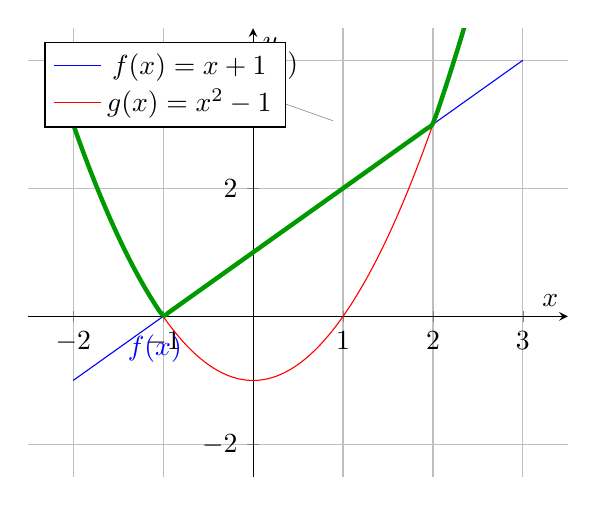
\begin{tikzpicture}
\begin{axis}[
    axis lines=middle,
    xlabel=$x$,
    ylabel={$y$},
    grid=major,
    xmin=-2.5, xmax=3.5,
    ymin=-2.5, ymax=4.5,
    legend pos=north west
]
% Les deux fonctions de base
\addplot[blue, smooth, domain=-2:3, samples=100] {x+1} node[pos=0.1, right] {$f(x)$};
\addplot[red, smooth, domain=-2:3, samples=100] {x^2-1} node[pos=0.9, right] {$g(x)$};

% Le maximum des deux fonctions
\addplot[green!60!black, ultra thick, smooth, domain=-2:3, samples=100] {max(x+1, x^2-1)};

\legend{$f(x)=x+1$, $g(x)=x^2-1$}
\node[pin=135:{$y=\max(f(x), g(x))$}] at (axis cs: 1,3) {};
\end{axis}
\end{tikzpicture}
\caption{La fonction $\max(f,g)$ (en vert) est continue si $f$ et $g$ le sont.}
\end{figure}

\begin{proof}
    Soit $x_0 \in I$. On veut montrer que $\max(f,g)$ est continue en $x_0$. Soit $\epsilon > 0$. On cherche $\delta > 0$ tel que :
    $$|x-x_0| < \delta \implies |\max(f(x),g(x)) - \max(f(x_0),g(x_0))| < \epsilon.$$
    On a :
    $$|\max(f(x),g(x)) - \max(f(x_0),g(x_0))| \leq |f(x) - f(x_0)| + |g(x) - g(x_0)|.$$
    Comme $f$ et $g$ sont continues en $x_0$, il existe $\delta_f > 0$ et $\delta_g > 0$ tels que :
    $$|x-x_0| < \delta_f \implies |f(x) - f(x_0)| < \frac{\epsilon}{2},$$
    $$|x-x_0| < \delta_g \implies |g(x) - g(x_0)| < \frac{\epsilon}{2}.$$
    On prend $\delta = \min(\delta_f,\delta_g)$. Alors, si $|x-x_0| < \delta$, on a :
    $$|\max(f(x),g(x)) - \max(f(x_0),g(x_0))| < \frac{\epsilon}{2} + \frac{\epsilon}{2} = \epsilon.$$
    Donc $\max(f,g)$ est continue en $x_0$. De même, on montre que $\min(f,g)$ est continue en $x_0$.
\end{proof}

\begin{property}
    Soit $a\in \mathbb{R}$ tel que $\forall \varepsilon > 0, a \leq \varepsilon$. Alors $a = 0$.

    \begin{proof}
    \textbf{Méthode 1 :} Supposons que $a \geq 0$, on prend $\varepsilon = \frac{a}{2} > 0$. Donc $a \leq \frac{a}{2}$, ce qui est absurde.\\
    \textbf{Méthode 2 :} On a $\forall \varepsilon > 0, \varepsilon - a \geq 0$. Donc $a$ est minorant sur $\mathbb{R}_+^*$. Donc $\inf(\mathbb{R}_+^*) \iff 0 \geq a$, et comme $a \geq 0$, on en déduit que $a=0$.
\end{proof}
\end{property}

\begin{consequence}
    Soit $a,b\in \mathbb{C}$ tels que : $\forall \varepsilon > 0, |a-b| \leq \varepsilon$. Alors $a=b$.
\end{consequence}

\chapter{Parties denses dans \(\mathbb{R}\)}

\section{Partie entière d'un réel}
\begin{definition}
    Soit $x \in \mathbb{R}$. La partie entière de $x$, notée $E(x)$ ou $\lfloor x \rfloor$, est le plus grand entier relatif inférieur ou égal à $x$.

    On peut aussi l'écrire : $E(x) = \max\{k \in \mathbb{Z}, k \leq x\}$.
\end{definition}

\begin{figure}[h!]
\centering
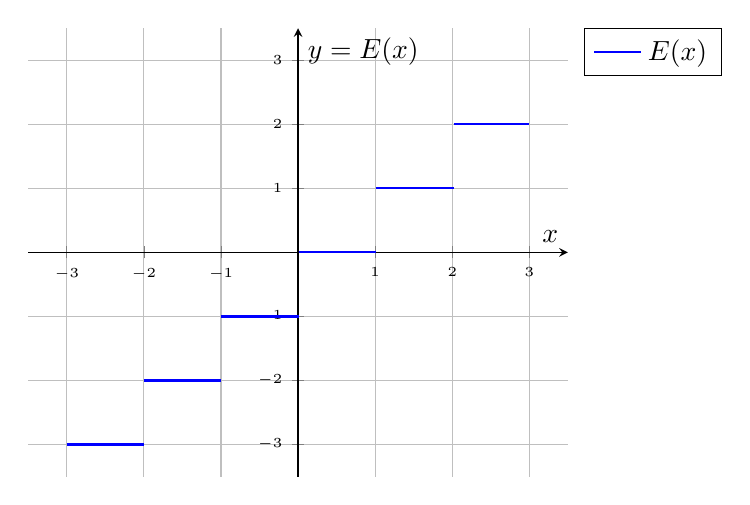
\begin{tikzpicture}
\begin{axis}[
    axis lines=middle,
    xlabel=$x$,
    ylabel={$y=E(x)$},
    grid=major,
    xmin=-3.5, xmax=3.5,
    ymin=-3.5, ymax=3.5,
    xtick={-3,-2,-1,0,1,2,3},
    ytick={-3,-2,-1,0,1,2,3},
    tick label style={font=\tiny},
    legend pos=outer north east
]
\addplot[
    blue, 
    thick, 
    domain=-3:3, 
    samples=300, 
    jump mark left % Style pour les fonctions en escalier
] {floor(x)};
\legend{$E(x)$}
\end{axis}
\end{tikzpicture}
\caption{Graphe de la fonction partie entière $f(x) = E(x)$.}
\end{figure}

\begin{remark}
    Soit $x \in \mathbb{R}$. Alors :
    \begin{itemize}
        \item $E(x) \leq x < E(x) + 1$.
        \item $x - 1 < E(x) \leq x$.
        \item $E(x) = n \iff n \leq x < n + 1$ pour $n \in \mathbb{Z}$.
        \item $E(x) = n \iff x - n \in [0,1[$ pour $n \in \mathbb{Z}$.
    \end{itemize}
\end{remark}

\begin{property}
    \quad
    \begin{enumerate}
        \item $\forall x \in \mathbb{R}, \forall m \in \mathbb{Z}, E(x+m) = E(x) + m$. Cette application est croissante.
        \item $\forall k\in\mathbb{Z}, \forall x\in [k,k+1[, E(x) = k$.
        \item $\forall x \in \mathbb{R}: E(x)=x\iff x \in \mathbb{Z}$.
        \item $\forall x \in \mathbb{R}, \forall k \in \mathbb{Z}, E(x+k) = E(x)+k$.
        \item $\forall x,y \in \mathbb{R} : \begin{cases}
        E(x)\leq x < E(x)+1\\
        E(y)\leq y < E(y)+1
        \end{cases} \\ \implies E(x)+E(y)\leq x+y < E(x)+E(y)+2 \\ \implies E(x+y) \in \{E(x)+E(y),E(x)+E(y)+1\}\\ \implies E(x+y)=E(x)+E(y) + E(x+E(x)+y-E(y))$.
        \item $\forall a,b \in \mathbb{R} / b-a > 1 : \exists k \in \mathbb{Z}, a < k < b$.
    \end{enumerate}
\end{property}

\begin{exercise}
    Résoudre dans $\mathbb{R}$ l'inéquation : $E(-x)=-E(x)$.
    \textbf{Solution :}\\
    Si $x \in \mathbb{Z}$, alors $E(-x)=-E(x)$, car $E(x)=x$ et $E(-x)=-x$.\\ Donc $Z \subset S$.\\
    Si $x \notin \mathbb{Z}$, alors $E(x) < x < E(x)+1$. Donc $-E(x)-1 < -x < -E(x)$. Donc $E(-x) = -E(x)-1$.\\Donc $x \notin S$.\\
    Donc $S = \mathbb{Z}$.
\end{exercise}

\section{Parties denses}

\begin{definition}[Partie dense]
Soit $\mathcal{D}$ une partie non vide de $\mathbb{R}$.
On dit que $\mathcal{D}$ est dense dans $\mathbb{R}$ lorsque pour tout couple $(u,v) \in \mathbb{R}^2$ tel que $u<v$, il existe un élément $d \in \mathcal{D}$ tel que $u < d < v$.
\end{definition}

\begin{proposition}
Les ensembles $\mathbb{Q}$ (nombres rationnels) et $\mathbb{R}\setminus\mathbb{Q}$ (nombres irrationnels) sont denses dans $\mathbb{R}$.

\begin{proof}[Preuve de la densité de $\mathbb{Q}$]
Soient $u, v \in \mathbb{R}$ avec $u < v$. On a donc $v-u > 0$.
Par la propriété d'Archimède, il existe un entier $q \in \mathbb{N}^*$ tel que $q > \frac{1}{v-u}$.
Ceci implique que $q(v-u) > 1$, soit $qv > qu+1$.
Les réels $qu$ et $qv$ sont donc distants de plus de 1. Il existe donc un unique entier $p \in \mathbb{Z}$ tel que $qu < p \le qu+1$.
On a alors $qu < p < qv$, et en divisant par $q$ (qui est strictement positif), on obtient $u < \frac{p}{q} < v$.
Nous avons trouvé un rationnel $\frac{p}{q}$ dans l'intervalle $]u,v[$, donc $\mathbb{Q}$ est dense dans $\mathbb{R}$.
\end{proof}

\begin{proof}[Preuve de la densité de $\mathbb{R}\setminus\mathbb{Q}$]
Soient $u, v \in \mathbb{R}$ avec $u < v$. On considère l'intervalle $]u-\sqrt{2}, v-\sqrt{2}[$.
Comme $\mathbb{Q}$ est dense dans $\mathbb{R}$, il existe un rationnel $r \in \mathbb{Q}$ tel que $u-\sqrt{2} < r < v-\sqrt{2}$.
En ajoutant $\sqrt{2}$, on obtient $u < r+\sqrt{2} < v$.
Posons $d = r+\sqrt{2}$. Le nombre $d$ est irrationnel. En effet, si $d$ était rationnel, alors $d-r = \sqrt{2}$ serait aussi rationnel (comme différence de deux rationnels), ce qui est absurde.
Nous avons trouvé un irrationnel $d$ dans l'intervalle $]u,v[$, donc $\mathbb{R}\setminus\mathbb{Q}$ est dense dans $\mathbb{R}$.
\end{proof}
\end{proposition}

\begin{proposition}[Caractérisation séquentielle de la densité]
Une partie $\mathcal{D}$ est dense dans $\mathbb{R}$ si et seulement si pour tout réel $x \in \mathbb{R}$, il existe une suite $(d_n)_n$ d'éléments de $\mathcal{D}$ qui converge vers $x$.
$$ \mathcal{D} \text{ dense} \iff \forall x \in \mathbb{R}, \exists (d_n)_n \in \mathcal{D}^{\mathbb{N}} \text{ t.q. } \lim_{n \to +\infty} d_n = x $$

\begin{proof}
($\Rightarrow$) Supposons $\mathcal{D}$ dense dans $\mathbb{R}$. Soit $x \in \mathbb{R}$. Pour tout $n \in \mathbb{N}^*$, on considère l'intervalle $I_n = ]x-\frac{1}{n}, x+\frac{1}{n}[$.
Puisque $\mathcal{D}$ est dense, il existe un élément $d_n \in \mathcal{D}$ dans cet intervalle. On a donc :
$$ \forall n \in \mathbb{N}^*, \quad x-\frac{1}{n} < d_n < x+\frac{1}{n} $$
Comme $\lim_{n \to \infty} (x-\frac{1}{n}) = \lim_{n \to \infty} (x+\frac{1}{n}) = x$, d'après le théorème des gendarmes, la suite $(d_n)_n$ converge vers $x$.

($\Leftarrow$) Supposons que pour tout réel $x$, il existe une suite d'éléments de $\mathcal{D}$ qui converge vers $x$. Soient $u,v \in \mathbb{R}$ avec $u<v$. Posons $x = \frac{u+v}{2}$.
Par hypothèse, il existe une suite $(d_n)_n$ d'éléments de $\mathcal{D}$ qui converge vers $x$.
Par définition de la convergence, pour $\varepsilon = \frac{v-u}{2} > 0$, il existe un rang $N \in \mathbb{N}$ tel que pour tout $n \ge N$, on a $|d_n - x| < \varepsilon$.
Ceci signifie que $x-\varepsilon < d_n < x+\varepsilon$. En remplaçant $x$ et $\varepsilon$ par leurs valeurs, on obtient :
$$ \frac{u+v}{2} - \frac{v-u}{2} < d_n < \frac{u+v}{2} + \frac{v-u}{2} \implies u < d_n < v $$
Nous avons trouvé un élément de $\mathcal{D}$ dans l'intervalle $]u,v[$, donc $\mathcal{D}$ est dense.
\end{proof}
\end{proposition}

\begin{example}
Pour tout $x \in \mathbb{R}$, la suite $(d_n)_n$ définie par $d_n = \frac{\lfloor nx \rfloor}{n}$ est une suite de nombres rationnels qui converge vers $x$.
En effet, on a l'encadrement $nx-1 < \lfloor nx \rfloor \le nx$, d'où $x-\frac{1}{n} < d_n \le x$. Par le théorème des gendarmes, $\lim_{n\to\infty} d_n = x$.
\end{example}

\section{Applications de la densité}

\begin{theorem}[Égalité de deux fonctions continues]
Soient $f$ et $g$ deux fonctions continues de $\mathbb{R}$ dans $\mathbb{R}$. Soit $\mathcal{D}$ une partie dense de $\mathbb{R}$.
Si $f$ et $g$ coïncident sur $\mathcal{D}$ (c'est-à-dire $\forall x \in \mathcal{D}, f(x)=g(x)$), alors $f$ et $g$ sont égales sur $\mathbb{R}$ tout entier.

\begin{proof}
Soit $x \in \mathbb{R}$. Puisque $\mathcal{D}$ est dense dans $\mathbb{R}$, il existe une suite $(d_n)_n$ d'éléments de $\mathcal{D}$ qui converge vers $x$.
Par hypothèse, pour tout $n \in \mathbb{N}$, on a $f(d_n) = g(d_n)$.
Comme les fonctions $f$ et $g$ sont continues sur $\mathbb{R}$, on peut utiliser la caractérisation séquentielle de la continuité :
$$ \lim_{n \to \infty} f(d_n) = f(\lim_{n \to \infty} d_n) = f(x) $$
$$ \lim_{n \to \infty} g(d_n) = g(\lim_{n \to \infty} d_n) = g(x) $$
Puisque les suites $(f(d_n))_n$ et $(g(d_n))_n$ sont égales, elles ont la même limite. Par unicité de la limite, on a donc $f(x)=g(x)$.
Ceci étant vrai pour n'importe quel $x \in \mathbb{R}$, on conclut que $f=g$.
\end{proof}
\end{theorem}




\begin{exercise}\quad
    \begin{itemize}
        \item Soit $f:\mathbb{R}\rightarrow\mathbb{R}$ une fonction continue sur $\mathbb{R}$ telle que : $\forall x \in \mathbb{R}, f(x)\sin(x)=0$. Montrer que $f\equiv0$.
        \item Déterminer l'ensemble des fonctions continues sur $\mathbb{R}$ telles que : $\forall x \in \mathbb{R}, f(x+y)=f(x)+f(y)$ (\textit{Equation de Cauchy}).
    \end{itemize}
    \textbf{Solution :}
    \begin{itemize}
        \item On pose $D=\{x\in\mathbb{R}, \sin(x)\not=0\}$. Donc $D=\mathbb{R}\setminus\{\pi n, n\in\mathbb{Z}\}$. On utilise la caractérisation séquentielle de la densité dans $\mathbb{R}$. On pose $a_n$ une suite définie telle que $\begin{cases}
        a_n=x \text{ si } x \in D\\
        a_n=k\pi+\frac{1}{n} \text{ sinon, avec } k\in\mathbb{Z} \text{ tel que } k\pi=x \text{ et } k\pi<k\pi+\frac{1}{n}< (k+1)\pi
        \end{cases}$
    \end{itemize}
\end{exercise}

\end{document}